\documentclass[reportComp]{thesis}
\usepackage[cpp,pseudo]{mypackage}

\title{模式识别作业一、二}
\subtitle{}
\school{数据科学与计算机学院}
\author{陈鸿峥}
\classname{17大数据与人工智能}
\stunum{17341015}
\headercontext{模式识别作业}
\lstset{language=python}

\begin{document}

\maketitle

\begin{question}[\textsection 2 Q2]
假设两个等概率的一维密度具有如下形式:对任给$i=1,2$及$0<b_i$,$p(x\mid\omega_i)\propto\ee^{-|x-a_i|/b_i}$。
\begin{itemize}
	\item [(a)] 写出每个密度的解析表达式,即对任意的$a_i$和正的$b_i$,将每个函数归一化
	\item [(b)] 计算似然比,作为$4$个变量的函数
	\item [(c)] 绘出在$a_1=0,b_1=1,a_2=1,b_2=2$时的似然比$p(x\mid\omega_1)/p(x\mid\omega_2)$的曲线图
\end{itemize}
\end{question}
\begin{answer}
\begin{itemize}
	\item [(a)] 设比例系数为$k_i$,由概率的基本性质有
\[\begin{aligned}
\qquad&\intab{-\infty}{\infty}{k_i\ee^{\frac{-|x-a_i|}{b_i}}}\\
=&\intab{-\infty}{a_i}{k_i\ee^{\frac{x-a_i}{b_i}}}+\intab{a_i}{\infty}{k_i\ee^{-\frac{x-a_i}{b_i}}}\\
=&2k_ib_i\\\
=&1
\end{aligned}\]
进而求得$k_i=1/(2b_i)$,故解析表达式为
\[p(x\mid\omega_i)=\frac{1}{2b_i}\ee^{-|x-a_i|/b_i}\]
	\item [(b)]
\[\frac{p(x\mid\omega_1)}{p(x\mid\omega_2)}=\frac{b_2}{b_1}\ee^{-\frac{|x-a_1|}{b_1}+\frac{|x-a_2|}{b_2}}\]
	\item [(c)]
将$a_1=0,b_1=1,a_2=1,b_2=2$代入(b)求得的式子化简得
\[\frac{p(x\mid\omega_1)}{p(x\mid\omega_2)}=2\ee^{-|x|+\frac{|x-1|}{2}}\]
图像如下
\begin{figure}[H]
\centering
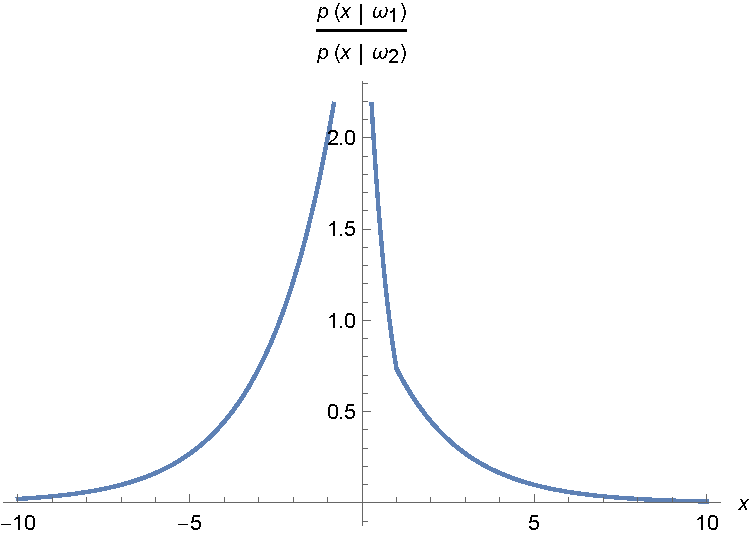
\includegraphics[width=0.5\linewidth]{likelihood.pdf}
\end{figure}
\end{itemize}
\end{answer}

\begin{question}[\textsection 2 Q7]
考虑两个一维柯西分布的Neyman-Pearson准则:
\[p(x\mid\omega_i)=\frac{1}{\pi b}\cdot\frac{1}{1+\lrp{\frac{x-a_i}{b}}^2}\,,\qquad i=1,2\]
在0-1误差损失下,且为了简化,设$a_2>a_1$,宽度$b$相同,且先验概率相等。
\begin{itemize}
	\item [(a)] 假设当一样本实际属于$\omega_1$却被误认为$\omega_2$的模式分类时的最大可接受误差率为$E_1$,用所给变量确定判决边界。
	\item [(b)] 对于此边界,将$\omega_2$错分为$\omega_1$的误差率是多少?
	\item [(c)] 在0-1损失率下的总误差率是多少?
	\item [(d)] 将你的结论应用于特殊情况:$b=1$且$a_1=-1,a_2=1$且$E_1=0.1$
	\item [(e)] 将你的结论与贝叶斯误差率(即没有Neyman-Pearson条件)作比较。
\end{itemize}
\end{question}
\begin{answer}
\begin{itemize}
	\item [(a)] 因先验概率相等,故$p(x\mid\omega_1)=1/2$。
	设判别边界为$x^\star$,则
	($\omega_1$曲线对应尖峰坐标为$a_1$,$\omega_2$曲线对应尖峰坐标为$a_2$,贝叶斯下交点右侧判为$\omega_2$)
	\[\begin{aligned}
	E_1&=\intab{x^\star}{\infty}{p(\omega_1\mid x)P(x)}\\
	&=\intab{x^\star}{\infty}{p(x\mid\omega_1)P(\omega_1)}\\
	&=\frac{1}{2}\intab{x^\star}{\infty}{\frac{1}{\pi b}\frac{1}{1+\lrp{\frac{x-a_1}{b}}^2}}\\
	&=\frac{1}{2\pi b}\intabu{u^\star}{\infty}{\frac{b}{1+u^2}}{u}\qquad u=\frac{x-a_1}{b}\\
	&=\frac{1}{2\pi}\arctan u\Big|_{u^\star}^{\infty}
	\end{aligned}\]
	移项得到
	\[2\pi E_1=\frac{\pi}{2}-\arctan\frac{x^\star-a_1}{b}\]
	两侧同时取$\tan$,整理得
	\[x^\star=a_1+\frac{b}{\tan(2\pi E_1)}\]

	\item [(b)] 由题(a)的结果
	\[\begin{aligned}
	E_2&=\intab{-\infty}{x^\star}{p(x\mid\omega_2)P(\omega_2)}\\
	&=\frac{1}{\pi b}\intab{-\infty}{x^\star}{\frac{1}{1+\lrp{\frac{x-a_i}{b}}^2}P(\omega_2)}\\
	&=\frac{1}{2\pi b}\intabu{-\infty}{u^\star}{\frac{b}{1+u^2}}{u}\qquad u=\frac{x-a_2}{b}\\
	&=\frac{1}{2\pi}\arctan u\Big|_{-\infty}^{u^\star}\\
	&=\frac{1}{4}+\frac{1}{2\pi}\arctan\frac{x^\star-a_2}{b}
	\end{aligned}\]
	
	\item [(c)] 综合题(a)和题(b)有
	\[E=E_1+E_2=E_1+\frac{1}{4}+\frac{1}{2\pi}\arctan\frac{x^\star-a_2}{b}\]
	
	\item [(d)] 将值代入(c)式得到$x^\star=0.3764$,$E=0.2613$
	
	\item [(e)] 由(d)的$a_1$和$a_2$对称知贝叶斯的决策边界为$x_B^\star=0$,进而贝叶斯误差率为
	\[\begin{aligned}
	E_B&=2\cdot\frac{1}{2\pi b}\intab{0}{\infty}{\frac{1}{1+\lrp{\frac{x-a_1}{b}}^2}}\\
	&=\arctan u\Big|_0^\infty\\
	&=0.25<E
	\end{aligned}\]
	即确实贝叶斯误差率会小于基于Neyman-Pearson准则的误差率
\end{itemize}
\end{answer}

\begin{question}[\textsection 2 Q9]
使用第7题给出的条件密度,设类别的先验概率相等。
\begin{itemize}
	\item [(a)] 证明最小误差概率为
	\[P(error)=\frac{1}{2}-\frac{1}{\pi}\tan^{-1}\left|\frac{a_2-a_1}{2b}\right|\]
	\item [(b)] 绘出它随$|a_2-a_1|/(2b)$变化的曲线图。
	\item [(c)] $P(error)$的最大值是多少?在什么条件下可以达到此值?试说明原因。
\end{itemize}
\end{question}
\begin{answer}
\begin{itemize}
	\item [(a)] 不妨设$a_2>a_1$,判决边界为$(a_1+a_2)/2$,则误差概率为
	\[\begin{aligned}
	P(error)&=\intab{-\infty}{(a_1+a_2)/2}{p(x\mid \omega_2)P(\omega_2)}+\intab{(a_1+a_2)/2}{\infty}{p(x\mid \omega_1)P(\omega_1)}\\
	&=\frac{1}{2\pi b}\lrp{\intab{-\infty}{(a_1+a_2)/2}{\frac{1}{1+\lrp{\frac{x-a_2}{b}}^2}}+\intab{(a_1+a_2)/2}{\infty}{\frac{1}{1+\lrp{\frac{x-a_1}{b}}^2}}}\\
	&=\frac{1}{2\pi b}\lrp{\arctan u\Big|_{-\infty}^{(a_1-a_2)/(2b)}+\arctan u\Big|_{(-a_1+a_2)/(2b)}^{\infty}}\\
	&=\frac{1}{2}-\frac{1}{\pi}\arctan\frac{a_2-a_1}{2b}
	\end{aligned}\]
	对于$a_1\leq a_2$的情形类似,故得证

	\item [(b)] 如下图所示
	\begin{figure}[H]
	\centering
	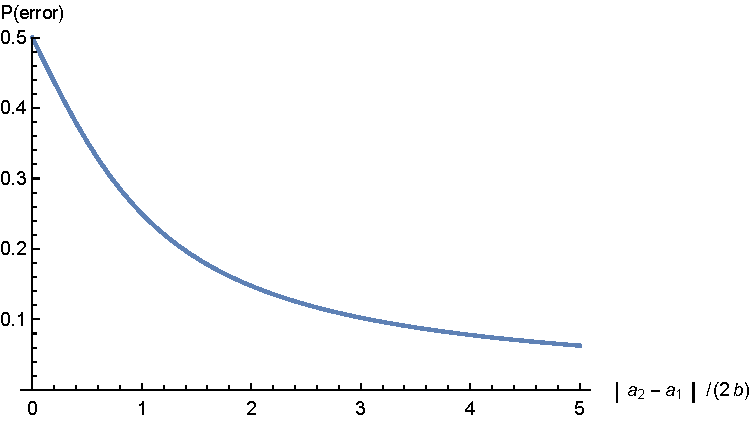
\includegraphics[width=0.5\linewidth]{error.pdf}
	\end{figure}

	\item [(c)] 当$|a_2-a_1|/(2b)=0$时$P(error)$达到最大值$1/2$,也即两个概率分布相同($a_1=a_2$),或者两个概率分布都为常量值($a_1\ne a_2,b=\infty$)
\end{itemize}
\end{answer}

\begin{question}[\textsection 2 Q23]
考虑三维正态分布$p(\vx\mid\omega)\thicksim N(\vmu,\Sigma)$,其中
\[\vmu=\bmat{1\\2\\2},\;\Sigma=\bmat{1 & 0 & 0\\0 & 5 & 2\\0 & 2 &5}\]
\begin{itemize}
	\item [(a)] 求点$\vx_0=\bmat{0.5 & 0 & 1}^\T$处的概率密度。
	\item [(b)] 构造白化变换$A_\omega=\phi\Lambda^{-1/2}$,计算分别表示本征向量和本征值的矩阵$\phi$和$\Lambda$;接下来,将此分布转换为以原点为中心协方差矩阵为单位阵的分布,即$p(\vx\mid\omega)\thicksim N(0,I)$。
	\item [(c)] 将整个同样的转换过程应用于点$\vx_0$以产生一变换点$\vx_\omega$。
	\item [(d)] 通过详细计算,证明原分布中从$\vx_0$到均值$\vmu$的Mahalanobis距离与变换后的分布中从$\vx_\omega$到$\vzero$\\的Mahalanobis距离相等。
	\item [(e)] 概率密度在一个一般的线性变换下是否保持不变?换句话说,对于某线性变换$T$,是否有$p(\vx_0\mid N(\vmu,\Sigma))=p(T^\T\vx_0\mid N(T^\T\vmu,T^\T\Sigma T))$?解释原因。
	\item [(f)] 证明当把一个一般的白化变换$A_\omega=\phi\Lambda^{-1/2}$应用于一个高斯分布时可保证最终分布的协方差与单位阵$I$成比例,检查变换后的分布是否仍然具有归一化特性。
\end{itemize}
\end{question}
\begin{answer}
\begin{itemize}
	\item [(a)] 我们有$d=3$维,
	\[|\Sigma|=\vmat{1 & 0 & 0\\0 & 5 & 2\\0 & 2 & 5}=21\]
	注意到$\Sigma$可表示为分块矩阵,我们有
	\[\Sigma=\bmat{1 &\vzero\\\vzero & A}\qquad A^{-1}=\bmat{5 & 2\\2 & 5}^{-1}=\bmat{5/|\det A| & -2/|\det A|\\-2/|\det A| & 5/|\det A|}=\bmat{5/21 & -2/21\\-2/21 & 5/21}\]
	进而
	\[\Sigma^{-1}=\bmat{1 & 0 & 0\\0 & 5 & 2\\0 & 2 & 5}^{-1}=
	\bmat{1 &\vzero\\\vzero & A^{-1}}=\bmat{1 & 0 & 0\\0 & 5/21 & -2/21\\0 & -2/21 & 5/21}\]
	故有平方Mahalanobis距离
	\[\begin{aligned}
	\qquad&(\vx_0-\vmu)^\T\Sigma^{-1}(\vx_0-\vmu)\\
	=&\bmat{0.5-1\\0-2\\1-2}^\T\bmat{1 & 0 & 0\\0 & 5/21 & -2/21\\0 & -2/21 & 5/21}\bmat{0.5-1\\0-2\\1-2}\\
	=& 1.06
	\end{aligned}\]
	将上述数值代入得到概率密度
	\[p(\vx_0\mid\omega)=\frac{1}{(2\pi)^{d/2}|\Sigma|^{1/2}}\exp\lrs{-\frac{1}{2}(\vx_0-\vmu)^\T\Sigma^{-1}(\vx_0-\vmu)}=0.008155\]

	\item [(b)] 先求出$\Sigma$的特征值,考虑特征方程$|\Sigma-\lambda I|=0$
	\[\vmat{1-\lambda & 0 & 0\\0 & 5-\lambda & 2\\0 & 2 & 5-\lambda}=(1-\lambda)(3-\lambda)(7-\lambda)=0\]
	对于不同特征值,回代求其特征向量,并可求得其通解形式
	\[\begin{aligned}
	\lambda_1&=1:\;\bmat{1 & 0 & 0\\0 & 5 & 2\\0 & 2 & 5}\bmat{x_1\\x_2\\x_3}=\bmat{x_1\\x_2\\x_3}\implies \vx=x_1\bmat{1\\0\\0}+x_2\bmat{0\\1\\-1}\\
	\lambda_2&=3:\;\bmat{1 & 0 & 0\\0 & 5 & 2\\0 & 2 & 5}\bmat{x_1\\x_2\\x_3}=3\bmat{x_1\\x_2\\x_3}\implies \vx=x_2\bmat{0\\1\\-1}\\
	\lambda_3&=7:\;\bmat{1 & 0 & 0\\0 & 5 & 2\\0 & 2 & 5}\bmat{x_1\\x_2\\x_3}=7\bmat{x_1\\x_2\\x_3}\implies \vx=x_2\bmat{0\\1\\1}\\
	\end{aligned}\]
	进而有三个正交基
	\[\begin{aligned}
	\phi_1 &=\bmat{1 & 0 & 0}^\T\\
	\phi_2 &=\bmat{0 & 1/\sqrt{2} & -1/\sqrt{2}}^\T\\
	\phi_3 &=\bmat{0 & 1/\sqrt{2} & 1/\sqrt{2}}^\T
	\end{aligned}\]
	最终得到正交特征向量矩阵
	\[\phi=\bmat{1 & 0 & 0\\0 & 1/\sqrt{2} & 1/\sqrt{2}\\0 & -1/\sqrt{2} & 1/\sqrt{2}}\]
	以及白化变换
	\[A_\omega=\phi\Lambda^{-1/2}=\bmat{1 & 0 & 0\\0 & 1/\sqrt{2} & 1/\sqrt{2}\\0 & -1/\sqrt{2} & 1/\sqrt{2}}\bmat{1 & 0 & 0\\0 & \sqrt{3} & 0\\0 & 0 & \sqrt{7}}=\bmat{1 & 0 & 0\\ 0 & 1/\sqrt{6} & 1/\sqrt{14}\\ 0 & -1/\sqrt{6} & 1/\sqrt{14}}\]
	进而有
	\[Y=A_\omega^\T(\vx-\vmu)\thicksim N(0,I)\]

	\item [(c)] 将$\vx_0$代入有
	\[\vx_\omega=A_\omega^\T(\vx_0-\vmu)=\bmat{1 & 0 & 0\\ 0 & 1/\sqrt{6} & -1/\sqrt{6}\\ 0 & 1/\sqrt{14} & 1/\sqrt{14}}\bmat{-0.5\\ -2\\ -1}=\bmat{-0.5\\-1/\sqrt{6}\\-3/\sqrt{14}}\]

	\item [(d)] 由(a)知原距离$r^2=1.06$,而新的距离
	\[r_\omega^2=\vx_\omega^\T I^{-1}\vx_\omega=\vx_\omega^\T\vx_\omega=1.06\]
	因此两者相等

	\item [(e)] 设线性变换后的向量为$\vx'=T^\T\vx$,进而有均值
	\[\vmu'=\sum_{k=1}^n\vx_k'\Big/n=\sum_{k=1}^n T^\T\vx_k\Big/n=T^\T\sum_{k=1}^n\vx_k\Big/n=T^\T\vmu\]
	和协方差
	\[\Sigma'=\sum_{k=1}^n(\vx_k'-\vmu')(\vx_k'-\mu')^\T=T^\T\lrs{\sum_{k=1}^n(\vx_k-\vmu)(\vx_k-\mu)^\T}T=T^\T\Sigma T\]
	进而
	\[p(\vx_0\mid N(\vmu,\Sigma))=p(T^\T\vx_0\mid N(T^\T\vmu,T^\T\Sigma T))\]

	\item [(f)] 由课本图2.8上面的公式,我们有
	\[p(A_\omega^\T\vx)\thicksim N(A_\omega^\T\vmu,A_\omega^\T\Sigma A_\omega)\]
	进而可得协方差矩阵(注意这里$\Sigma=\phi\Lambda\phi^\T$是基于谱分解/特征分解)
	\[\begin{aligned}
	A_\omega^\T\Sigma A_\omega &= (\phi\Lambda^{-1/2})^\T\phi\Lambda\phi^\T(\phi\Lambda^{-1/2})\\
	&= \Lambda^{-1/2}(\phi^\T(\phi\Lambda\phi^\T)\phi)\Lambda^{-1/2}\\
	&= I
	\end{aligned}\]
	故变换后的分布依然具有归一化特性
\end{itemize}
\end{answer}

\end{document}